\documentclass{wileySix}
\usepackage{w-bookps}

% \usepackage{mathptmx}

\usepackage{graphicx}
\usepackage{enumitem}

\setcounter{secnumdepth}{3}

\setcounter{tocdepth}{2}

\begin{document}

\booktitle{Web Service}
\subtitle{Semua Tentang Komunikasi antar Aplikasi Berbasis Protokol internet}

\author{Rolly Maulana Awangga}

\halftitlepage
\titlepage



\offprintinfo{Web Service, pre-release}{Rolly Maulana Awangga}


\begin{copyrightpage}{2018}
Web Service / Rolly Maulana Awangga
\end{copyrightpage}


\dedication{For my family}

\contentsinbrief %optional
\tableofcontents
\listoffigures %optional
\listoftables  %optional

%%%%%%%%%
%%Content 
%%%%%%%%%

\part[Pengenalan Web Service]
{Pengenalan\\ Web Service}

%\chapter[Contoh]
%{Contoh\\ Latex}
%\prologue{The sheer volumne of answers can often stifle insight...The purpose
of computing\index{computing!the purpose} is insight, not numbers.}
{Hamming}

\section{Definisi Web Service}
Web service adalah suatu sistem perangkat lunak yang dirancang untuk mendukung interoperabilitas dan interaksi antar sistem pada suatu jaringan. Web service digunakan sebagai suatu fasilitas yang disediakan oleh suatu web site untuk menyediakan layanan (dalam bentuk informasi) kepada sistem lain, sehingga sistem lain dapat berinteraksi dengan sistem tersebut melalui layanan-layanan (service) yang disediakan oleh suatu sistem yang menyediakan web service. Web service menyimpan data informasi dalam format XML, sehingga data ini dapat diakses oleh sistem lain walaupun berbeda platform, sistem operasi, maupun bahasa compiler.

Web service bertujuan untuk meningkatkan kolaborasi antar pemrogram dan perusahaan, yang memungkinkan sebuah fungsi di dalam Web Service dapat dipinjam oleh aplikasi lain tanpa perlu mengetahui detil pemrograman yang terdapat di dalamnya.

Beberapa alasan mengapa digunakannya web service  adalah sebagai berikut:

-Web service dapat digunakan untuk mentransformasikan satu atau beberapa bisnis logic atau class dan objek yang terpisah dalam satu ruang lingkup yang menjadi satu, sehingga tingkat keamanan dapat ditangani dengan baik. 

-Web service memiliki kemudahan dalam proses deployment-nya, karena tidak memerlukan registrasi khusus ke dalam suatu sistem operasi. Web service cukup di-upload ke web server dan siap diakses oleh pihak-pihak yang telah diberikan otorisasi.

-Web service berjalan di port  80 yang merupakan protokol standar HTTP, dengan demikian web service tidak memerlukan konfigurasi khusus di sisi firewall.\cite{awangga2017colenak}.

\section{Sejarah Web Service}
Penemu website adalah Sir Timothy John ¨Tim¨ Berners-Lee, sedangkan website yang tersambung dengan jaringan, pertamakali muncul pada tahun 1991. Maksud dari Tim ketika membuat website adalah untuk mempermudah tukar menukar dan memperbarui informasi kepada sesama peneliti di tempat dia bekerja. Pada tanggal 30 April 1993, CERN (tempat dimana Tim bekerja) menginformasikan bahwa WWW dapat digunakan secara gratis oleh semua orang. Sebuah website bisa berupa hasil kerja dari individu, atau menunjukkan kepemilikan dari sebuah organisasi, perusahaan, dan biasanya website itu menujukkan beberapa topik khusus, atau kepentingan tertentu. Sebuah website bisa berisi hyperlink yang menghubungkan ke website lain, jadi, kadang sulit membedakan antara website yang dibuat oleh individu perseorangan dengan website yang dibuat oleh organisasi bisnis bisa saja tidak kentara.

Website yang ditulis di konversi menjadi HTML oleh komputer dan diakses melalui web browser, yang dikenal juga dengan HTTP Client. Halaman web dapat dilihat atau diakses melalui jaringan komputer dan internet, perangkatnya bisa saja berupa komputer pribadi, laptop, PDA ataupun telepon selular.

Sebuah website dibuat didalam sebuah sistem komputer yang dikenal dengan server web, juga disebut HTTP Server, dan pengertian ini juga bisa menunjuk pada software yang dipakai untuk menjalankan sistem ini, yang kemudian menerima lalu mengirimkan halaman-halaman yang diperlukan untuk merespon permintaan dari pengguna. Apache adalah piranti lunak yang biasa digunakan dalam sebuah webserver, kemudian setelah itu adalah Microsoft Internet Information Services.



\subsection{Sir Timothy John ¨Tim¨ Berners-Lee}
Pada tanggal 30 April 1993, CERN (tempat dimana Tim bekerja) menginformasikan bahwa WWW dapat digunakan secara gratis oleh semua orang.

\begin{figure}[ht]

\centerline{\includegraphics[width=1\textwidth]{figures/petaduniaalid.JPG}}
\caption{Gambaran pengantar peta dunia karya al-Idrisi tahun 1154.}
\end{figure}

\begin{figure}[ht]
	\centerline{\includegraphics[width=1\textwidth]{figures/TabulaRogeriana.jpg}}
\vskip2pt
\caption{Tabula Rogeriana digambar oleh Al-Idrisi pada tahun 1154 untuk Raja Normandia Roger II dari Sisilia, setelah delapan menetap di istananya, di mana dia bekerja untuk penjelasan dan ilustrasi peta.}
\end{figure}




%\chapter[Internet]
%{Definisi\\ Internet}
%\input{section/1internet.tex}

%\chapter[Web]
%{Definisi\\ Web}
%\documentclass[12pt, a4paper]{article}
\linespread{1.5}


\title{World Wide Web}
\maketitle

%\begin{itemize}
%\item Imron Sumadireja (1164076)
%\item Jesron Marudut (1164077)
%\item Lusia Violita Aprilian (1164080)
%\item Mhd. Zulfikar Akram Nst. (1164081)
%\end{itemize}

\section{Pengertian Website}
World wide web (www atau web) merupakan halaman situs informasi yang dapat diakses secara cepat atau sarana
antar muka informasi di internet. Web dapat menggabungkan teks, grafik, dan multimedia. Web memudahkan
penggunanya untuk mengakses informasi melalui konsep hypertext sehingga memungkinkan  suatu text untuk
menjadi acuan membuka dokumen laindo. Informasi dapat mudah disebar dan diakses.

\subsection{Sejarah Website}
Sementara itu World wide web (www) dikembangkan pertama kali oleh Tim Berners-Lee pada tahun 1989. Pada
awalnya, Tim mengusulkan WWW sebagai suatu cara berbagai dokumen diantara para peneliti. Dokumen online dapat
diakses melalui alamat unik yang disebut Universal Resource Locator atau URL. Selain itu WWW tidak hanya
dikembangkan untuk keperluan para peneliti, namun juga dikembangkan untuk kalangan pendidikan, bisnis dan
perorangan. Berdasarkan penjelasan singkat diatas dapat disimpulkan bahwa antara web dan internet memiliki
hubungan yang sangat erat walaupun keduangnay tidak bisa dikatakan sama. Web merupakan bagian dari layanan
yang dapat berjala di atas teknologi internet.

\subsection{Jenis-jenis website}
Website dikelompokan dalam beberapa jenis-jenis Website agar dapat memudahkan dalam menentukan jenis website
yang akan ditentukan. Dan berikut jenis-jenis website yang dikelompokan atas beberapa dasar:
\begin{enumerate}
\item Jenis Website berdasarkan sifat;
\begin{itemize}
\item Website Statis, merupakan web yang kontenya hampir jarang diubah
\item Website Dinamis, Web yang konten atau isinya dapat berubah-ubah setiap saat
\end{itemize}
\item Jenis Website yang dikelompokkan berdasarkan Bahasa Pemrogramannya;
\begin{itemize}
\item Server side, Website yang memakai bahasa pemrograman yang tergantung dengan servernya
\item Client side, adalah web yang tidak perluu server untuk menjalankannya. Cukup diakses dengan browser.
\end{itemize}
\item Jenis-jenis Web menurut tujuannya;
\begin{itemize}
\item Web personal, biasanya web ini merupakan web yang berisi informasi seorang
\item Corporate Web, website yang dimiliki sebuah institusi atau perusahaan.
\item Web Portal, Web ini berisi banyak layanan, seperti berita, email dan jasa
\item Web Forum, sebuah web yang dibuat sebagai sarana diskusi.
\end{itemize}
\end{enumerate}
	
\subsection{Keuntungan Web}
Keuntungan penggunaan web diantaranya yaitu :
\begin{itemize}
\item Informasi dapat diberikan segera(tepat waktu) dan diperbarui secara berkala.
\item Presentasi fleksible dan visibilitas dapat menyediakan ragam isyarat untuk diseminasi informasi.
\item Informasi dapat diorganisir melalui tautan dan menu, berbagai tingkatan informasi dapat disediakan format file yang berbeda dapat digunakan untukj informasi yang dapat diunduh. Integrasi informasi dapat dilakukann melalui tautan dan seksi lain, halaman lain, atau web lain.
\item Tauta  dan menu dapat menyediakan informasi bagi pemangku kepentingan yang berbeda, informasi dapat pula diberikan melalui daftar email kepada pemangku kepentingan.
\item Setiap orang yang dapat mengakses web dapat memperoleh informasi karena keterjangkauan global dan potensi komunikasi masl dari web.
\end{itemize}
	   
\section{tentang web scraping}
Web scraping atau scraping web (dapat disebut juga panen web atau web ekstraksi data) merupakan sebuah
perangkat lunak komputer teknik penggalian informasi dari situs web seperti mengambil mengambil data
berbentuk teks yang umumnya bertipe HTML atau XHTML. contohnya seperti Internet Explorer (IE) dan Mozilla Web
Browser. web scraping berkaitan erat dengan pengindekan web.

\subsection{manfaat dari web scraping}
Web scraping sering dikenal dengan screen scraping. Web scraping tidak dapat dimasukkan kedalam bidang data
mining karena dalam data mining menyiratkan upaya untuk memahami pola semantik dari sejumlah data besar yang
telah diperoleh. Aplikasi Web scraping hanya fokus pada cara memperoleh data melalui pengambilan dan ekstrasi
dengan ukuran data yang bervariasi. Manfaat dari web scraping adalah agar informasi yang diambil lebih
terfokus sehingga dapat memudahkan dalam melakukan pencarian sesuatu, adapun cara untuk mengembangkan teknik
web scraping yaitu dengan cara sebagai berikut:
\begin{enumerate}
\item Pengembang/pembuat program mempelajari dokumen HTML dari website yang akan diambil informasinya untuk
di tag HTML tujuannya yakni untuk mengapit informasi yang akan diambil (Create Scraping Template)
\item Pengembang/pembuat program mempelajari teknik navigasi pada website yang akan diambil informasinya
untuk ditiru pada aplikasi web scraping yang akan dibuat (Explore Site Navigation)
\item Selanjutnya aplikasi web scraping akan mengotomisasi informasi yang didapatkan dari website yang telah
ditentukan (Automate Navigation and Extraction), informasi yang didapat tersebut akan disimpan dalam 
tabel basis data (Extracted Data and Package History).
\end{enumerate}

\subsection{Perbandingan Metode Web Scraping}
Berikut perbandingan antara metode Web Scraping menggunakan CSS Selector dan Xpath Selector
\begin{enumerate}
\item Penggunaan metode XPATH Selector untuk web scraping menghasilkan artikel yang lebih lengkap
dibandingkan dengan menggunakan metode CSS Selector, Ditunjukkan dengan jumlah item dan ukuran file
yang didapatkan lebih besar. Namun juga menyisakan proses lain untuk menghilangkan kode HTML yang tidak
diinginkan dari artikel yang dihasilkan menggunakan metode XPATH Selector.
\item Dalam penggunaan memori baik metode XPATH Selector dan CSS Selector tidak memiliki perbedaan yang
signifikan(cenderung sama). Disebabkan karena engine scrapy yang baik dalam penggunaan resource-nya. 
\item Metode XPATH Selector memiliki waktu proses yang lebih cepat daripada menggunakan metode CSS Selector.
\item Pada metode XPATH, selector cukup mengikuti node pada halaman web, sehingga waktu yang dibutuhkan
relatif lebih singkat.
\end{enumerate}

\section{Tentang Web Hosting}
Web hosting merupakan jasa penyewaaan tempat penyimpanan data di internet atau biasa disebut dengan cloud
yang diperlukan oleh sebuah website. Web hosting ialah salah satu syarat agar website bisa diakses secara 
online dan dapat diakses dari seluruh dunia. Ukuran yang digunakan dalam suatu web hosting adalah kapasitas
dan bandwidth. Kapasistas merupakan ukuran besarnya kemampuan sebuah web hosting untuk menyimpan data-data di internet.

Bandwidth merupakan ukuran maksimal dari jumlah volume data yang diperbolehkan untuk diakses dari web hosting
setiap bulannya. Sebagai contoh, sebuah halaman website yang mempunyai ukuran 2 MB dan bandwidth web hosting
2000 MB, maka setiap bulannya website tersebut dapat diakses sebanyak 2000 kali.

\subsection{Tentang Domain}
Domain merupakan sebuah alamat di dunia internet atau sebuah identitas dari sebuah website. Domain digunakan untuk mempermudah dalam mengakses situs yang ada di internet. Domain terbagi menjadi 2 jenis domain yang dibagi berdasarkan pemisahaan titiknya, yaitu; Top Level Domain (TLD) dan Second Level Domain (SLD). Top Level Domain merupakan bagian terakhir dalam sebuah domain website. Contohnya "facebook.com" dan disitu yang jadi domainnya adalah ".com". Selanjutnya Second Level Domain atau SLD merupakan bagian dari domain yang terdapat sebelum Top Level Domain. Contohnya "Facebook.com" yang menjadi SLDnya adalah Facebook. Jadi SLD adalah unsur domain yang didaftarkan terdahulu pada jasa Web Hosting. Dan ada juga yang disebut Country Code Second Level Domain (ccSLD). Berguna sebagai penunjuk organisasi apa yang mendaftar pada suatu domain. Setiap negara juga mempunyai ccSLD yang berbeda-beda tiap negaranya.

\subsection{Tentang Hubungan Domain dan Web Hosting}
Hubungan Domain dan Web Hosting merupakan satu kesatuan yang saling membutuhkan. Pada sebuah Website, domain dan web hosting saling ketergantungan. Apabila yang tersedia hanya web hosting, maka website tidak akan dapat diakses. Begitu juga dengan domain, apabila yang tersedia hanya domain, maka tidak akan ada website yang akan ditampilkan, karena halaman website tersimpan didalam web hosting.

\subsection{Macam-macam Web Hosting}
Saat ini banyak jasa penyedia hosting dengan harga relatif murah bahkan gratis. Berikut adalah macam-macam web hosting :
\begin{enumerate}
\item Free Hosting / Web Hosting Gratis
Dengan free hosting, kita dengan mudah mencari layanan web hosting dan domain gratis di internet dengan menggunakan fasilitas search engine seperti google atau yang lainnya. Biasanya penyedia web hosting tidak mengenakan biaya. Namun, memiliki banyak keterbatasan beberapa fitur.
\item Web Hosting Berbagi atau Shared Hosting
Jenis hosting ini paling sering digunakan karena bukan hanya murah, namun juga memiliki layanan yang  dapat mencukupi segala kebutuhan. Biasanya, untuk menggunakan layanan web hosting ini anda hanya perlu untuk mengeluarkan biaya sebesar 100 hingga 200 ribu untuk mendapatkan ruang sebesar 2 GB – 7,5 GB dengan bandwith unlimited.
\item VPS Web Hosting
VPS merupakan singkatan dari Virtual Private Server. Jadi disini anda dapat seperti memiliki server sendiri untuk situs anda. dengan server ini, anda akan memiliki control yang lebih dalam seperti Dedicated Server.
\item Dedicated Web Hosting
Dedicated Web Hosting merupakan sebuah layanan hosting dengan server yang memiliki kemampuan untuk melakukan handle terhadap traffic dengan jumlah sangat banyak. Serta memiliki banyak fitur premium di dalamnya. Selain itu,juga memiliki control penuh terhadap server walaupun  hanya menyewanya.
\item Managed Web Hosting
Managed Hosting / Web Hosting Terkelola ini adalah web hosting yang dikhususkan untuk situs dengan. Platform yang sama. Managed web hosting biasanya lebih aman dan kinerjanya lebih optimal. Selain itu, memudahkan untuk melakukan beragam pengaturan, mulai dari installasi, sampai setting macam-macamnya.
  \end{enumerate}

\subsection{Cara Mendapatkan Web Hosting dan Domain}
Web hosting dan domain lebih sering ditemukan oleh perusahaan-perusahaan penyedia web hosting atau domain. Untuk menemukannya, cukup cari di google. Maka akan banyak perusahaan yang menyediakan jasa web hosting. Kinerja web hosting berbeda-beda dari setiap perusahaan Web hosting. Karna apabila web hosting yang dibuat oleh jasa tersebut buruk maka website tersebut akan mudah bermasalah. Oleh karena itu dalam pembelian jasa domain atau web hosting perlu diperhatikan hal-hal seperti profil dari penjual web hosting, fitur untuk website dan harga dari web hosting tersebut. Dalam memilih penyedia web hosting, pastikan penyedia mempunyai reputasi yang bagus dan terpercaya. Dan sebaiknya memilih perusahaan web hosting yang sudah dalam bentuk perusahaan CV atau PT agar pertanggung jawabannya jelas ketika terjadi gangguan web hosting.
	
\section{Apa itu cPanel?}
Apa itu cPanel?
cPanel adalah perangkat lunak control panel online untuk melakukan pengaturan website dalam sebuah web histing. cPanel adalah tool utama untuk pengguna web hosting. 
Beberapa fungsi utama cPanel antara lain yaitu upload data website, pengaturan data website, instalasi content management system, dan lain-lain. Melelui cPanel juga kita bisa mengatur data-data website. Kita bisa menambah, menghapus, atau memodifikasi data website.

\subsection{Backup date dengan cPanel}
Kemudahan yang diberikan cPanel sebagai control panel yakni untuk mempermudah proses hosting di suatu situs web menggunakan 3 tingkatan struktur untuk memberikan fungsi administrator, agen, dan yang memiliki situs web tersebut untuk mengatur berbagai macam aspek dari situs web dan administrasi server melalui sebuah web standar. Dalam menu cPanel untuk backup disediakan 3 pilihan layanan backup yang ada yakni:
\begin{enumerate}
\item System Backup, merupakan menu backup yang dapat digunakan untuk mendownload backup otomatis yang telah dibuat oleh administrator server
\item Full Backup, akan melakukan backup file untuk mengembalikan file yang corrupt, terhapus atau pindah pada server yang lain.
\item Backup Home Directory, berfungsi untuk memberikan hak akses untuk mengambil file yang berada pada directory home.
\end{enumerate}


\chapter[Backend]
{Definisi\\ Backend}


\section{Backend}

\begin{figure}[ht]
\centerline{\includegraphics[width=1\textwidth]{figures/1backend.jpg}}
\caption{Backend}
\label{1backend}
\end{figure}

	Pada gambar \ref{1backend} berikut ini dijelaskan mengenai Back-end atau server-side yang merupakan bagaimana sebuah website berkerja, meng-update
dan berubah. back-end adalah sesuatu system yang dimana User tidak akan dapat melihatnya di dalam browser,
seperti Database dan Server. biasanya orang - orang yang bekerja di bagian back-end di panggil atau disebut sebagai
Programmers atau Developer. Back-end developers adalah orang yang paling khawatir tentang hal - hal yang menyangkut keamanan,
struktur sistem dan manajemen konten. sebenarnya para back-end develper juga mengetahui tentang front-end seperti HTML dan CSS.
namun itu bukanlah bidang mereka bekerja. 

\subsection{Backend System}
	Pada system dan metode  yang membuat informasi dapat digunakan secara oromatis untuk mengakses 
pada fungsionalitas system computer backend yang digunakan ke server aplikasi. 
Metode ini juga dapat beroperasi untuk menghubungkan ke system computer backend dan memperoleh 
fungsionalitas untuk menentukan informasi  pada system backend. Dan pada informasi yang diperoleh 
dan dapat dianalisis secara terprogram,dan informasi yang sangat baru dapat dianalisis yang dimana 
informasi dibuat secara terprogram dapat digunakan untuk mengakses fungsionalitas system backend.
Back-end biasanya mengacu pada program dan skrip yang bekerja di dalam server, untuk membuat sebuah 
halaman web yang dinamis dan interatif. Back-end memiliki tugas-tugas yaitu seperti :

\begin{enumerate}
\item Desain Informasi pada web
\item Pemrosesan form
\item Pemrograman dalam database
\item Aplikasi Berbasis Web
\end{enumerate}
Dari tugas - tugas tersebut Back-end memiliki tiga bagian diantaranya yaitu server,aplikasi, dan database
\cite{shapiro2005system}.

\section{Bahasa Pemrograman yang digunakan di Backend}
Pada gambar \ref{2labelgambar} berikut ini dijelaskan bahwa pada Backend terdapat beberapa bahasa programing yang digunakan,
termasuk C, Python, dan lainnya. pada materi di bawah ini terdapat beberapa penjelasan tentang bahasa pemrogramannya.

\begin{figure}[ht]
\centerline{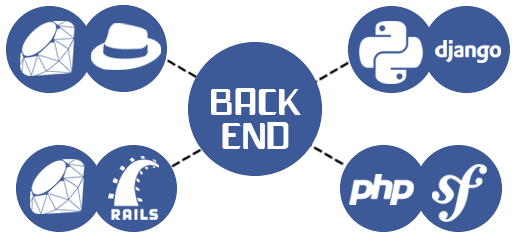
\includegraphics[width=1\textwidth]{figures/1bahasapemrogramanbackend.png}}
\caption{Bahasa Pemrograman yang dipakai di Backend}
\label{2labelgambar}
\end{figure}

\subsection{C}
	Bahasa Pemrograman Backend yang biasa digunakan developer ialah C, C++, dan Java .
Bahasa C adalah suatu perkembangan dari bahasa B yang di kembangkan oleh Ken Thompson pada tahun 1980.
Bahasa C rilis pertama kali ditulis oleh Brian W. Bahasa C, awalnya digunakan oleh sistem operasi UNIX.
Bahasa C adalah bahasa pemrograman tingkat standar, bahasa C memiliki kegunaan yang sering di gunakan
diantaranya untuk membuat perangkat lunak.

\subsection {C++}
	Pengertian C++ adalah `multi-paradigm' artinya anda dapat menulis suatu kode, caranya procedural 
tapi juga bisa menggunakan fungsional,berorientasi objek, dan campuran paradigm suatu pemrograman.  
Bahasa pemrograman C++ ini bisa lebih sulit untuk dipelajari; kita dapat mengembangkan dengan 
menggunakan satu atau lebih dari model ini,  atau kita dapat menggabungkan dengan Bahasa pemrograman lainnya.

\subsection {C\#}
	Sedangkan C\# merupakan sebuah bahasa programming yang simple, modern, OOP dan aman untuk 
penggabungannya dengan beberapa bahasa programming lain
\cite{hejlsberg2003c}.

\subsection {PHP}
 	adalah salah satu server side untuk dirancang khusus untuk aplikasi web dan PHP disisipkan diantara bahasa HTML sebab bahasa server side, maka dieksekusi diserver. sehingga yang kirimkan ke browser adalah hasil jadi dalam bentuk HTML. PHP termasuk Open Source Product dapat diubah disource code dan mendistribusikan secara bebas.

\subsection{Python}
	Python merupakan  bahasa pemrograman yang serba guna atau bersifat open source. 
Python lebih menekankan pada pembacaan  kode agar lebih mudah untuk memahami sintaks. 
Hal tersebut membuat bahasa pemrograman python lebih mudah dipelajari baik pemula maupun untuk yang 
sudah menguasai bahasa pemrograman ini dan dilengkapi dengan fungsionalitas standar besar serta 
komprehensif. Pyhton telah digunakan untuk mengembangkan berbagai macam perangakat lunak, seperti 
internet scipting, system programming, user interfaces, prudect customization,numberic programming. 
Pada saat ini bahasa pemrograman pyhton menduduki posisi 4 atau 5 paling sering digunakan diseluruh dunia.

\subsection{Perl}
	Proxy server ialah suatu komputer atau beberapa komputer yang diletakkan sebagai pelayanan kepada pelanggan yang ingin mengajukan layanan data baik dari pusat komputer(server).
Proxy server sering disebut sebagai media cache terhadap suatu konten website. Di ruang lingkup pendidikan pada laboratorium komputer jaringan di Institusi Sains \& Teknologi ditemukan jaringan yang belum ada penanganan masalah internet yang diakses berkali-kali sehingga bandwidth pada internet tidak efektif, penelitian ini bertujuan  untuk melakukan suatu penyimpanan konten yang diakses ke dalam proxy server kemudian melakukan filter konten menggunakan pemrograman PERL.
Ini dilakukan melalui proxy server, yaitu melalui fungsi pada cachig dan filter pada proxy server dengan menggunakan pemrograman PERL dan regex pada PERL
\cite{pamungkas2017implementasi}.

\subsection{ASP .NET}
	ASP.NET merupakan produk dari teknologi Microsoft untuk pengembangan aplikasi berbasis web dinamis. 
Bahasa pemrograman ini mempermudah pada pemula maupun yang sudah menguasai bahasa pemrograman ini , dikarenakan memberikan solusi pada pengembang untuk mendesign aplikasi web dengan cepat, mudah dan efisien. 
ASP diproses melalui web server dan menghasilkan HTML untuk dikirimkan pada web browser.


\subsection{Java}
	Dalam backend juga menggunaka javascript yaitu suatu format teks untuk mengserialisasi data yang terstruktur yang berasal dari objek literal JavaScripts.Pada JavaScript dapat mewakili dari empat tipe yaitu string, angka, boolean, dan nul, dan ada juga dua tipe terstruktur yaitu objek dan array. Objek kumpulan yang tanpa batas dari nol ata lebih dari nama atau nilai pasangannya, yang dimana nama ialah string sedangkan nilai ialah angka, boolean, objek, dan null. Array yaitu urutan dari nol atau melebihi banyak nilai.

\subsection{Ruby}
	Ruby merupakan bahasa pemrograman yang stabil, dengan menggabungkan bahasa pemrograman favoritnya seperti Perl, smalltalk, Eiffel, dan Lisp.
Membentuk suatu bahasa pemrograman baru yang menyeimbangkan pemrograman fungsional dengan imperatif.
Bahasa pemrograman Ruby mempunyai sistem yang dengan otomatis akan langsung terhapus semua data-data yang tidak terpakai dan tidak digunakan lagi pada memori. 
Platform sistem operasi yang mendukung bahasa pemrograman Ruby yaitu sistem operasi Linux, Unix, Amiga, Symbian, Mac dan Windows.

\section{Database Backend}
	Pada sistem basis data yaitu telah lama dilanda masalah kinerja pada penigkatan dalam penggunaan mainframe atau di dalam aplikasi basis data. Dan solusi untuk masalah ini yaitu dengar membongkar sistem basis data dari komputer mainframe ke komputer backend. Pada komputer itu memiliki penyimpanan disk sendiri, digunakan juga untuk melakukan semuoa operasi data base, dan saling berinteraksi dengan mainframe
\cite{yousefi2008database}.


\section{Arsitektur Three-Tier}
	Didalam masalah arsitektur two-tier telah diupdate ke tingkat tertentu dengan memperluas dari dua tingkat menjadi tiga tingkat.
Arshitektur three-tier akan mengisolisasi pemrosesan data dari lokasi pusat yang dapat dengan mudah diubah tanpa melibatkan dan mepengaruhi klien. Di dalam arsitektur three-tier ini, logika presentasi berada pada tingkat pertama (klien), logika bisnis berada pada 
tingkat menengah, dan yang lainnya seperti database berada di tingkatan ketiga yaitu back-end. Di tingkat menengah dalam
arsitektur three -tier (server aplikasi) akan menangani pemrosesan data dan akan menjadi antarmuka antara front - end (klien) dan
tingkat back-end (database)
\cite{demurjian1986multi}.


\section{Web Service}
	Web Service merupakan penyatuan dari 2 aspek yaitu Web dan Service, yang mana penjelasan Web dan Service akan dijelaskan di bawah ini :

\subsection{Web}
	pertama - tama disini akan dijelaskan tentang Web, Web merupakan website yang berarti 
jaringan yang dapat mengakses situs secara global.

\subsection{Service}
	Service merupakan layanan, yang dimana digunakan untuk melayani dan melakukan pelayanan.
sehingga dari kedua perihal diatas dapat disimpulkan bahwasanya web service adalah sebuah jaringan global yang memiliki pelayanan atau keamanan,
didalam web service user diberikan layanan berupa keamanan dalam berselancar di Internet. 
macam - macam model dari web service adalah sebagai berikut ini :

\begin{enumerate}
\item SOAP (Simple Object Access Protocol)
\item WDSL (Web Service Description Language)
\item RDF (Resource Description Framework)
\item RSS (Really Simple Syndication)
\end {enumerate}
\cite{curbera2001web}.


\section{Backend Developer}
	Orang yang bekerja di bagian back-end atau bisa kita sebut seorang back-end developer adalah seorang programmer yang hanya
memusatkan atau berfokus pada bagian keamanan, desain sistem, dan management data pada sistem. Seorang back-end developer
sangat dibutuhkan dalam melakukan pengembangan sistem atau sebuah aplikasi yang dinamis atau aplikasi yang memiliki data selalu
berubah - ubah, contohnya website yang dinamis seperti facebook dan google.

\section{Backend as a Service}
	Baas adalah sebuah provider untuk web dan mobile app developer untuk dapat mengkoneksikan 
aplikasi mereka ke dalam system penyimpanan cloud backend sekaligus masih tetap melakukan proses yang lain seperti user management, 
mendapatkan notifikasi, bermain social media, dan fitur – fitur lainnya yang terdapat di dalam aplikasi mobile mereka saat ini.

\subsection{Kelebihan yang dimiliki BaaS}
	Tujuan dari BaaS adalah untuk membuat hidup developer menjadi 
lebih mudah. BaaS ada karena kurangnya keahlian dari seorang 
mobile developer dan tingginya tingkat permintaan user untuk 
aplikasi smartphone mereka. berikut ini adalah kelebihannya :

\begin{enumerate}
\item Keuntungan yang efisien
\item Lebih cepat waktu penjualannya
\item Aplikasi didelivery dengan sumber daya yang lebih sedikit
\item Ter-optimisasi untuk mobile dan tablet
\item Aman dan terukur
\item Penggunaan sumber daya API yang umum dipakai
\end{enumerate}

\subsection {Yang dapat anda buat dengan menggunakan BaaS}
\begin{enumerate}
\item Pengembangan Website
\item Mobile Aplikasi, dll
\end{enumerate}
\cite{lane2015overview}.

\section{JSON (JavaScript Object Notation)}
	merupakan sebuah format pertukaran data yang mudah dibaca atau dimengerti dan dituliskan oleh manusia, 
serta JSON memiliki kemudahan untuk diterjemahkan dan juga diubah \(generate\) oleh sebuah mesin \(Computer\).
JSON adalah sebuah format teks yang tidak memiliki ketergantugan pada Bahasa pemrograman manapun karena JSON menggunakan 
gaya penulisannya sendiri yang mana dia menggunakan Bahasa – Bahasa pemrograman yang sudah umum seperti C family, Java, 
JavaScript, Perl, Python dan lainya, dan menjadikannya sebagai sebuah format yang tetap miliknya sendiri.
hal tersebutlah yang menjadikan JSON sebagai format pertukaran data yang ideal didalam dunia pemrograman
\cite{crockford2006application}.


\section{Mobile Backend Starter}
	Backend tidak hanya dipakai oleh web yang dinamis namun akhir - akhir ini google telah menambahkan sebuah layanan yang bernama
`Mobile Backend Starter', google menambahkan layanan tersebut dengan tujuan untuk memudahkan pengguna untuk menggunakan
layanan awan berupa `Cloud Services' dalam sebuah aplikasi mobile yang akan dikembangkan. Ketersediaan dari layanan `Mobile Backend Starter' ini bebas digunakan untuk publik
\cite{soinu2014cloud}.



		



\chapter[Frontend]
{Frontend}
\input{section/1Frontend.tex}

% contoh aplikasi web service
% web service
% protokol
% port

% HTTP
% URL
% POST
% GET


\bibliographystyle{IEEEtran}.
\bibliography{references}.

\printindex

\end{document}
